%----------------------------------------------------------------------------------------
%	PACKAGES AND DOCUMENT CONFIGURATIONS
%----------------------------------------------------------------------------------------
\documentclass[11pt]{article}
\usepackage{amsmath} % Required for some math elements
\usepackage{hyperref} 
\usepackage{xcolor}
\usepackage{lipsum} 
\usepackage{cite}
\usepackage{graphicx} % Required for the inclusion of images
\usepackage{algorithmic}
\usepackage{array}
\usepackage{bookmark}
\usepackage{listings}
\usepackage{amssymb}
\usepackage{enumitem}
\usepackage{pythonhighlight}
\usepackage[T1]{fontenc}
\usepackage{inconsolata}
\usepackage[margin=8mm]{geometry}
\usepackage[caption=false, font=footnotesize]{subfig}
\usepackage{fancyhdr}
\pagestyle{fancy}
\renewcommand{\headrulewidth}{0.4pt}
\renewcommand{\footrulewidth}{0.4pt}

\usepackage[active,tightpage]{preview}
\renewcommand{\PreviewBorder}{1in}
\newcommand{\Newpage}{\end{preview}\begin{preview}}
  


\newlist{steps}{enumerate}{1}
\setlist[steps, 1]{label = Step \arabic*:}

\hypersetup{ %color attributes of citation, link, etc.
    colorlinks=true,
    linkcolor=blue,
    filecolor=gray,      
    urlcolor=blue,
    citecolor=blue,
}

\newcommand{\matlab}{\textsc{Matlab }} %very important and totally necessary addition
\newcommand{\hdotrule}[1]{\hbox to \textwidth{\leaders\hbox to #1pt{\hss . \hss}\hfil}}

\newcommand\Item[1][]{%
  \ifx\relax#1\relax  \item \else \item[#1] \fi
  \abovedisplayskip=0pt\abovedisplayshortskip=0pt~\vspace*{-\baselineskip}}
%----------------------------------------------------------------------------------------
%	DOCUMENT INFORMATION
%----------------------------------------------------------------------------------------

\title{ECEN 405 \\ Lab 2: Power converters (Part 1 - Synchronous buck converter) Submission}
\author{Daniel Eisen : 300447549}
\date{\today}

\begin{document}
\begin{preview}

      \maketitle
      \hrule
      %----------------------------------------------------------------------------------------
      %	DOCUMENT CONTENT
      %----------------------------------------------------------------------------------------
      \section{Output Filter}
      $V_{in}=30V,\; V_{out}=20,\; f_{sw}=22kHz,\; R_{L}=100\Omega$
            \begin{center}
                  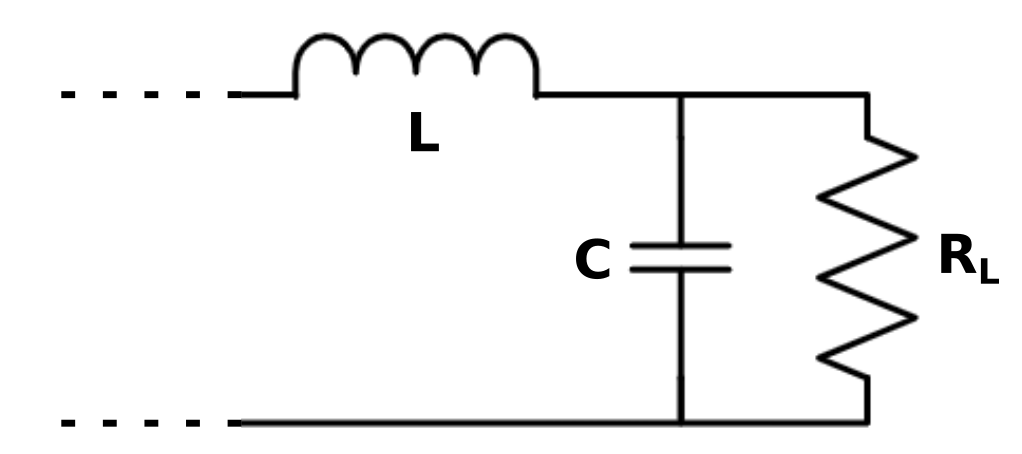
\includegraphics[height=0.2\textwidth]{img/filter.png}
            \end{center}
            $$D=\frac{V_{out}}{V_{in}} = 0.66\bar{6}, \; V_{os}=0.05V_{out}=1V$$
            $$I_{L}=\frac{V_{out}}{R_{L}}0.2A, \; I_{ripple}=0.4I_{L} = 0.08A, \; I_{max}=I_{L}+\frac{I_{ripple}}{2} = 0.24$$
            $$L=\frac{V_{out}\cdot\left(1-D\right)}{f_{sw}\cdot I_{ripple}}=0.003\bar{78}=3.78mH$$
            $$C=\frac{I_{max}^{2}\cdot L}{\left(V_{o}+V_{os}\right)^{2}-V_{o}^{2}}=0.0000053215=5.32\mu F$$
      \subsection{Discontinuous Conduction Frequency}
            $$f_{d}=\frac{R_{L}\left(1-D\right)}{2L} = 4400Hz$$
      \section{Deadtime Resistance}
            From datasheet: \\
            $R_{DT}=0 \rightarrow DT=0.4\mu S$ \\
            $R_{DT}=200k \rightarrow DT=5\mu S$
            $$\frac{\mu S}{k\Omega} = \frac{5-0.4}{200} = 0.023$$
            $$R_{DT} = \frac{0.5-0.4}{0.023} = 4.3478k\Omega$$

            Deadtime, in the context on MOSFET gate driving, is the time between 1 FET's gate is switched off and the other is turned on. This prevents the circumstance when (the FETs being in series between V+ and GND without resistance) both FETS are on due to switching delays and causes a short. 
      \section{Constant Output}
            The filtering capacitance smooths the high frequency PWM output and the VL varies dependant on Vin to meet constant output voltage.
      \section{Waveforms}
            \begin{center}
                  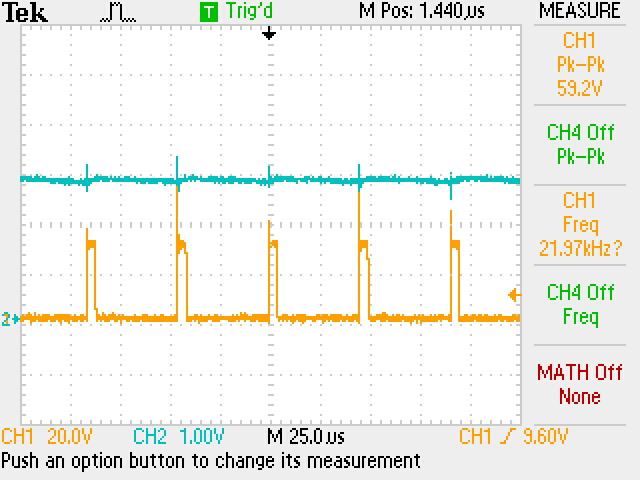
\includegraphics[height=0.2\textwidth]{img/10perc_duty_output.JPG}
                  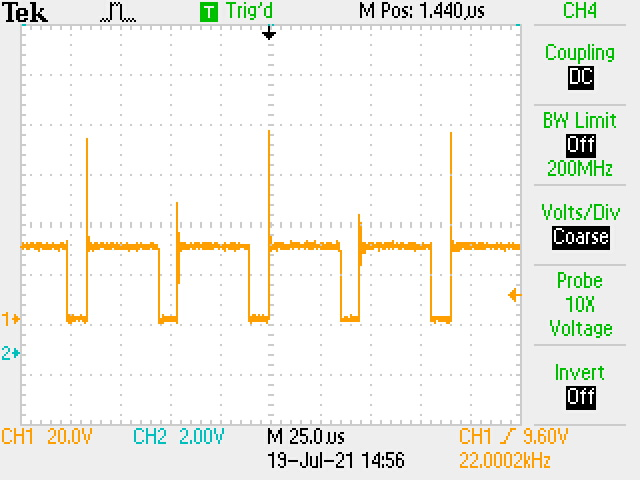
\includegraphics[height=0.2\textwidth]{img/80perc_dut.JPG}
            \end{center}
            The waveforms above are captured from the S-D junction of the FETs, Ie the output, and shows the pulse width modulated signal of the Vo = 20V at both 10 and 80 percent.
      \section{Efficiency vs Output Current}
            \begin{center}
                  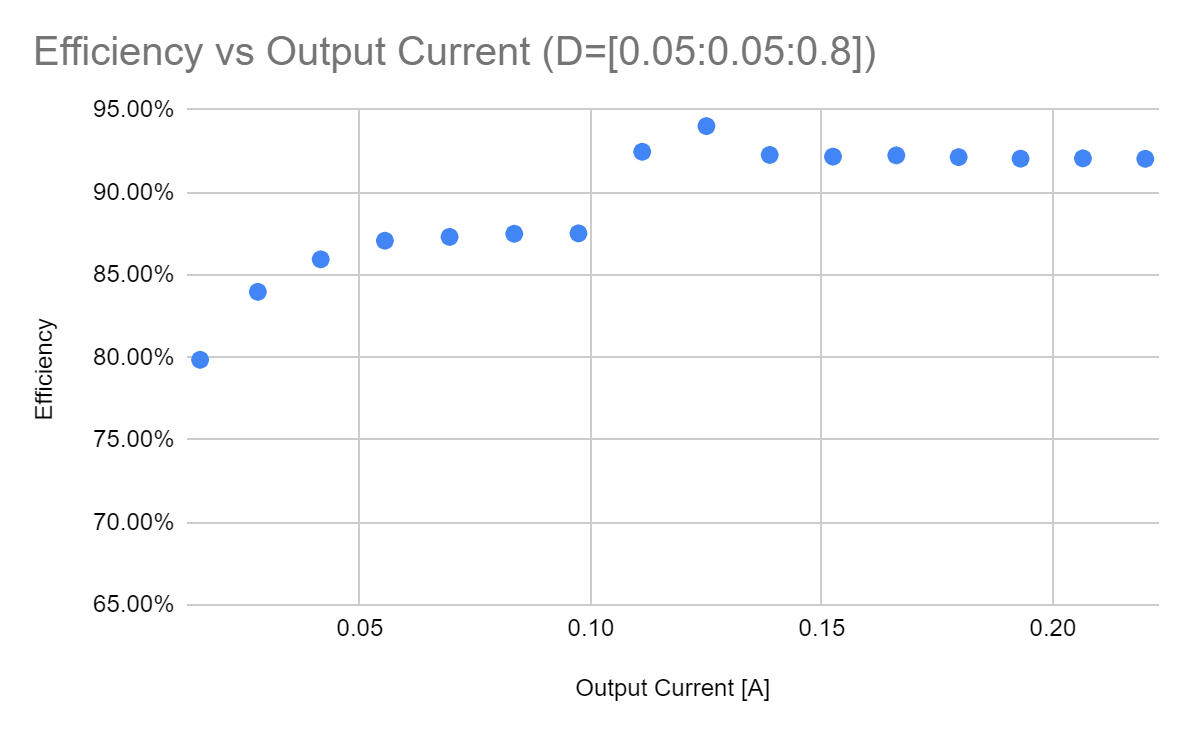
\includegraphics[height=0.3\textwidth]{img/eff.png}
            \end{center}
      \section{Bootstrap Circuit}
            The bootstrap circuit provides a positive bias for the high-side gate driver. This provides the correct reference to enable the gate to be switched on when the high-side driver is active. 

      \hrule
\end{preview}
\end{document}